\chapter{Faster scheduling heuristics}
\label{chap:schedulingHeuristics}

Determination of an optimal schedule requires traversal of an entire state-transition graph for programs, what takes an exponential computation time with a number of programs and other parameters. To make schedules computation faster, we also propose two heuristics: ``random walk" and ``greedy" \-- which however result in suboptimal schedules. Anyway, later in Chapter~\ref{chap:evaluation} we demonstrate that some heuristic performs almost as an optimal approach, but takes drastically less time to be computed. 

\begin{figure*}
\center
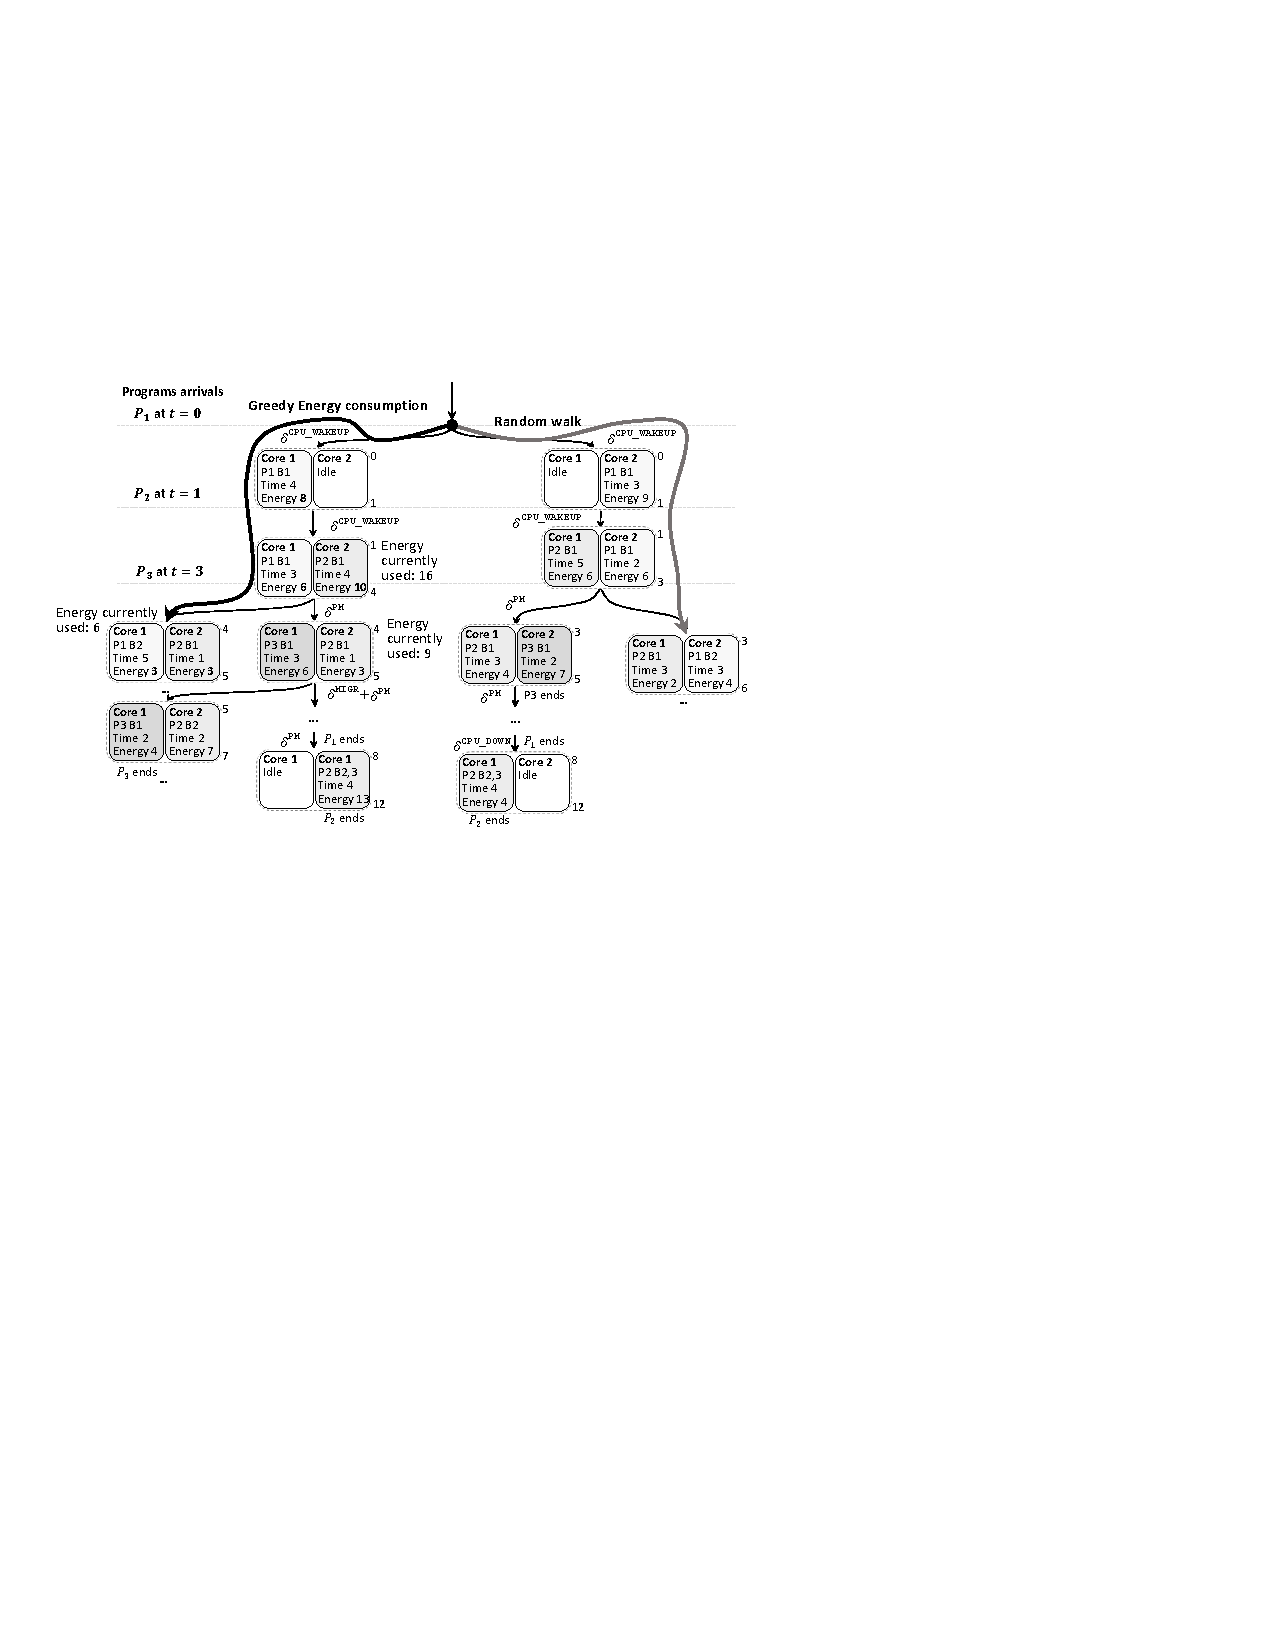
\includegraphics[width=.9\textwidth]{figs/greedyAndRandomWalk.pdf}
\caption{Greedy energy consumption and random walk traversals of a joint state-transition graph. Non-preemptive case.}
\label{fig:greedyAndRandomWalk}
\end{figure*}

Fig.~\ref{fig:greedyAndRandomWalk} demonstrates greedy and random walk applied to a joint-state-transition graph traversal. Below we provide some details on these heuristics, and later in Chapter~\ref{chap:evaluation} we evaluate their scheduling performance.

\section{Random walk}
\label{sec:randomWalk}

Using a random walk heuristic all scheduling decisions are made randomly without any particular knowledge about graph states. For a given graph state, the next state to be examined is chosen randomly among successors. This procedure continues until a graph leaf state is reached producing a certain schedule. In a $K$-random walks heuristic, this random walk is repeated $K$ times producing $K$ schedules. As a result the most optimal schedule is chosen.


\section{Greedy walk}
\label{sec:greedyWalk}

In a greedy walk locally optimal scheduling decisions are made. Given a graph state, the neighbouring state with a certain greedy-metric optimized is picked. Such a metric of a graph state can be its total blocks required execution time, energy consumption, number of migrations and preemptions, energy-delay product, and other. The greedy walk completes at a graph leaf state resulting in a certain suboptimal schedule. As a greedy-metric we chose graph state completion time, which minimizes of both total response time and energy-delay product.

